\documentclass[tikz,border=8pt]{standalone}
% Shared look for every TikZ diagram. Load with % Shared look for every TikZ diagram. Load with % Shared look for every TikZ diagram. Load with \input{../../tools/tikz-style.tex}
\usepackage[T1]{fontenc}
\usepackage{lmodern}
\renewcommand{\sfdefault}{lmr}  % diagrams use the same serif as the text
\usetikzlibrary{arrows.meta, positioning, shapes.geometric, calc, fit, backgrounds}
\definecolor{cblue}{HTML}{4C78A8}
\definecolor{corange}{HTML}{F58518}
\definecolor{cgreen}{HTML}{54A24B}
\definecolor{cred}{HTML}{E45756}
\definecolor{cpurple}{HTML}{B279A2}
\definecolor{cgrey}{HTML}{6B6B6B}
\tikzset{
  every picture/.style={font=\sffamily, line width=1.2pt},
  box/.style={draw=#1, fill=#1!12, rounded corners=4pt, align=center, inner sep=7pt, minimum height=1.1cm},
  box/.default=cgrey,
  arrow/.style={-{Stealth[length=3mm]}, draw=cgrey, line width=1.4pt},
  title/.style={font=\sffamily\bfseries\Large},
  note/.style={font=\sffamily\small, text=cgrey, align=center},
}
\AtBeginDocument{\hyphenpenalty=10000 \exhyphenpenalty=10000}

\usepackage[T1]{fontenc}
\usepackage{lmodern}
\renewcommand{\sfdefault}{lmr}  % diagrams use the same serif as the text
\usetikzlibrary{arrows.meta, positioning, shapes.geometric, calc, fit, backgrounds}
\definecolor{cblue}{HTML}{4C78A8}
\definecolor{corange}{HTML}{F58518}
\definecolor{cgreen}{HTML}{54A24B}
\definecolor{cred}{HTML}{E45756}
\definecolor{cpurple}{HTML}{B279A2}
\definecolor{cgrey}{HTML}{6B6B6B}
\tikzset{
  every picture/.style={font=\sffamily, line width=1.2pt},
  box/.style={draw=#1, fill=#1!12, rounded corners=4pt, align=center, inner sep=7pt, minimum height=1.1cm},
  box/.default=cgrey,
  arrow/.style={-{Stealth[length=3mm]}, draw=cgrey, line width=1.4pt},
  title/.style={font=\sffamily\bfseries\Large},
  note/.style={font=\sffamily\small, text=cgrey, align=center},
}
\AtBeginDocument{\hyphenpenalty=10000 \exhyphenpenalty=10000}

\usepackage[T1]{fontenc}
\usepackage{lmodern}
\renewcommand{\sfdefault}{lmr}  % diagrams use the same serif as the text
\usetikzlibrary{arrows.meta, positioning, shapes.geometric, calc, fit, backgrounds}
\definecolor{cblue}{HTML}{4C78A8}
\definecolor{corange}{HTML}{F58518}
\definecolor{cgreen}{HTML}{54A24B}
\definecolor{cred}{HTML}{E45756}
\definecolor{cpurple}{HTML}{B279A2}
\definecolor{cgrey}{HTML}{6B6B6B}
\tikzset{
  every picture/.style={font=\sffamily, line width=1.2pt},
  box/.style={draw=#1, fill=#1!12, rounded corners=4pt, align=center, inner sep=7pt, minimum height=1.1cm},
  box/.default=cgrey,
  arrow/.style={-{Stealth[length=3mm]}, draw=cgrey, line width=1.4pt},
  title/.style={font=\sffamily\bfseries\Large},
  note/.style={font=\sffamily\small, text=cgrey, align=center},
}
\AtBeginDocument{\hyphenpenalty=10000 \exhyphenpenalty=10000}

\begin{document}
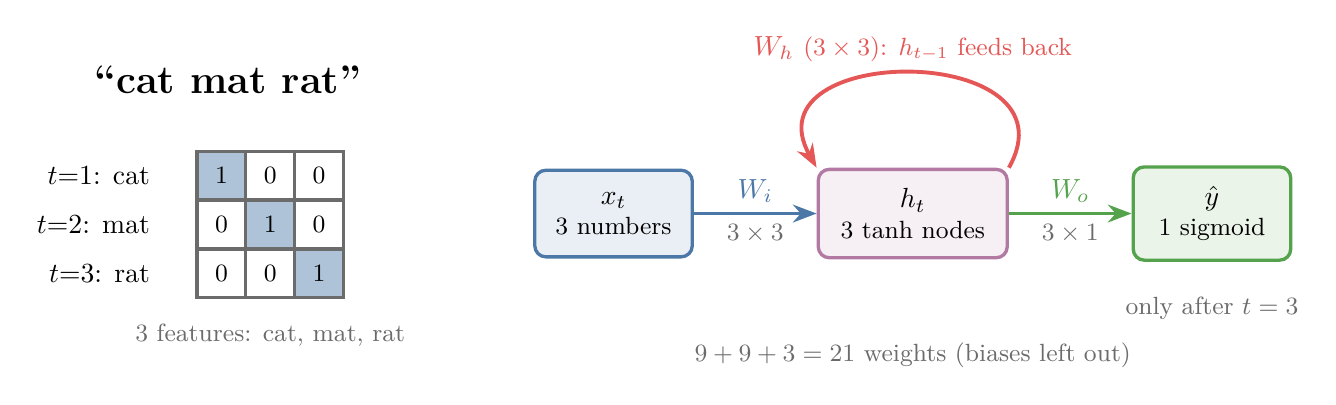
\begin{tikzpicture}[cell/.style={draw=cgrey, minimum size=0.62cm, inner sep=0pt, font=\sffamily\small},
  on/.style={cell, fill=cblue!45}, off/.style={cell, fill=white}]
  % one review as a 3x3 table: rows = time steps, columns = features
  \node[title] at (0.7,1.7) {``cat mat rat''};
  \foreach \w/\a/\b/\c [count=\r] in {cat/1/0/0, mat/0/1/0, rat/0/0/1} {
    \node[anchor=east, font=\sffamily] at (-0.15,1.1-0.62*\r) {$t{=}\r$: \w};
    \foreach \v [count=\k] in {\a,\b,\c} {
      \ifnum\v=1 \node[on] at (0.62*\k,1.1-0.62*\r) {1}; \else \node[off] at (0.62*\k,1.1-0.62*\r) {0}; \fi
    }
  }
  \node[note] at (1.24,-1.55) {3 features: cat, mat, rat};
  % network
  \node[box=cblue, minimum width=2.0cm] (x) at (5.6,0) {$x_t$\\[-1pt]\small 3 numbers};
  \node[box=cpurple, minimum width=2.4cm] (h) at (9.4,0) {$h_t$\\[-1pt]\small 3 tanh nodes};
  \node[box=cgreen, minimum width=2.0cm] (y) at (13.2,0) {$\hat{y}$\\[-1pt]\small 1 sigmoid};
  \draw[arrow, draw=cblue] (x) -- node[above, text=cblue] {$W_i$} node[below, note] {$3 \times 3$} (h);
  \draw[arrow, draw=cgreen] (h) -- node[above, text=cgreen] {$W_o$} node[below, note] {$3 \times 1$} (y);
  \draw[arrow, draw=cred] (h.north east) .. controls +(0.9,1.6) and +(-0.9,1.6) .. node[above, text=cred] {$W_h$\ \small($3 \times 3$): $h_{t-1}$ feeds back} (h.north west);
  \node[note] at (13.2,-1.2) {only after $t = 3$};
  \node[note] at (9.4,-1.8) {$9 + 9 + 3 = 21$ weights (biases left out)};
\end{tikzpicture}
\end{document}
